%%%%%%%%%%%%%%%%%%%%%%%%%%%%%%%%%%%%%%%%%%%%%%%%%%%%%%%%%%%%
%%  This Beamer template was created by Cameron Bracken.
%%  Anyone can freely use or modify it for any purpose
%%  without attribution.
%%
%%  Last Modified: January 9, 2009
%%

\documentclass[xcolor=x11names,compress, graphics]{beamer}
\usepackage{etex}
%% General document %%%%%%%%%%%%%%%%%%%%%%%%%%%%%%%%%%
\usepackage{graphicx}
\usepackage{tikz}
\usetikzlibrary{decorations.fractals}
%%%%%%%%%%%%%%%%%%%%%%%%%%%%%%%%%%%%%%%%%%%%%%%%%%%%%%
\usepackage{movie15}
\usepackage{float}
\usepackage{subfig}
\usepackage{amsmath}
\usepackage{amsfonts}
\usepackage{mathrsfs}
\usepackage{mathtools}

\usepackage{algorithm, algorithmic}

%% Beamer Layout %%%%%%%%%%%%%%%%%%%%%%%%%%%%%%%%%%
\useoutertheme[subsection=false,shadow]{miniframes}
\useinnertheme{default}
\usefonttheme{serif}
\usepackage{palatino}

\setbeamerfont{title like}{shape=\scshape}
\setbeamerfont{frametitle}{shape=\scshape}

\setbeamercolor*{lower separation line head}{bg=DeepSkyBlue4} 
\setbeamercolor*{normal text}{fg=black,bg=white} 
\setbeamercolor*{alerted text}{fg=red} 
\setbeamercolor*{example text}{fg=black} 
\setbeamercolor*{structure}{fg=black} 
 
\setbeamercolor*{palette tertiary}{fg=black,bg=black!10} 
\setbeamercolor*{palette secondary}{fg=black,bg=black!10}
\setbeamercolor*{palette quaternary}{fg=black,bg=black!10} 

%% Set the background and font color of the blocks 
\setbeamercolor{block title}{bg=DeepSkyBlue4,fg=white}

%% Set the type of the blocks
\setbeamertemplate{blocks}[shadow=true]

\newcommand{\topline}{%
  \tikz[remember picture,overlay] {%
    \draw[DeepSkyBlue4] ([yshift=-1.5cm, xshift = 1cm]current page.north west)
             -- ([yshift=-1.5cm,xshift=\paperwidth-1cm]current page.north west);}}
             
\setbeamertemplate{section in toc}[sections numbered]           

\renewcommand{\(}{\begin{columns}}
\renewcommand{\)}{\end{columns}}
\newcommand{\<}[1]{\begin{column}{#1}}
\renewcommand{\>}{\end{column}}

\usepackage[skip=10pt,font=scriptsize]{caption}
\captionsetup[figure]{labelformat=empty}

\DeclarePairedDelimiter\floor{\lfloor}{\rfloor}

\makeatother
\setbeamertemplate{footline}
{
  \leavevmode%
  \hbox{%
  \begin{beamercolorbox}[wd=.4\paperwidth,ht=2.25ex,dp=1ex,center]{author in head/foot}%
    \usebeamerfont{author in head/foot}\insertshortauthor
  \end{beamercolorbox}%
  \begin{beamercolorbox}[wd=.6\paperwidth,ht=2.25ex,dp=1ex,center]{title in head/foot}%
    \usebeamerfont{title in head/foot}\insertshorttitle\hspace*{3em}
    \insertframenumber{} / \inserttotalframenumber\hspace*{1ex}
  \end{beamercolorbox}}%
  \vskip0pt%
}
\makeatletter
%%%%%%%%%%%%%%%%%%%%%%%%%%%%%%%%%%%%%%%%%%%%%%%%%%

\title{\scshape \textbf{C Basics}}
\author{\scriptsize\scshape Angel No\'e Mart\'inez Gonz\'alez}


\usepackage{listings}

\begin{document}

% The title page
\begin{frame}
\setcounter{framenumber}{1}
\titlepage
\scriptsize

\end{frame}
%===============


\section[\scshape Data Types]{\scshape Data Types}
\begin{frame}[allowframebreaks]{Data Types}
\topline

The memory can be viewed as a {\color{red}bytes} serie, directionable components; each byte has their unique direction in memory (32 bits in 32 bits machine)

\begin{figure}
    \begin{center}
        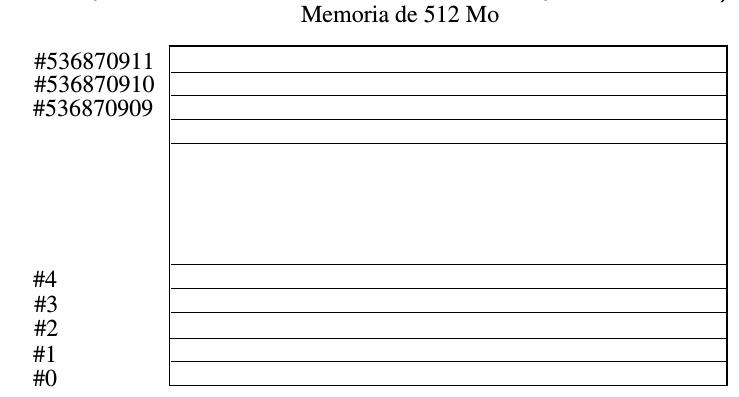
\includegraphics[width=7cm]{figures/memory_directions.jpeg}
    \end{center}
\end{figure}

\framebreak
\topline

\begin{itemize}
    \item Generally speaking, a k-bits system has registers and buses of k-bits. We can have a system manipulator of 32 bits on a OS of 64 bits but not otherwise.
    \item A data type defines: number of bytes to use for a data and the way to use each byte.
    \item Elemental types: \textbf{characters}, \textbf{integers} and \textbf{floating points} (for real numbers).
    \item There is no standard in data types size but
    $$
    \begin{array}{c}
    \text{1} == \text{sizeof(char)} \leq \text{sizeof(short)} \leq \text{sizeof(int)}\leq\\ \text{sizeof(float)} \leq \text{sizeof(double)} \leq \text{sizeof(long double)}    
    \end{array}
    $$    
\end{itemize}

\textit{sizeof(x)} returns the bytes number of the variable x: variable type or only type. 

\framebreak
\topline

In a 32 bits machine

\begin{figure}
    \begin{center}
        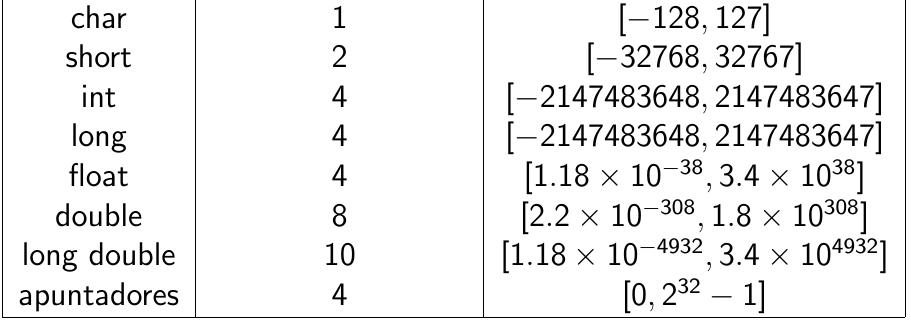
\includegraphics[width=10cm]{figures/types_range.jpeg}
    \end{center}
\end{figure}
    
\textit{unsigned} of a type take only the positive values.

\end{frame}


\begin{frame}[allowframebreaks]{Integer Types}
\topline

To represent a subset on $\mathbb{N}$

\begin{figure}
    \begin{center}
        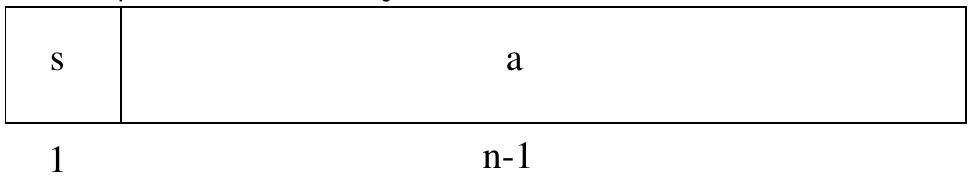
\includegraphics[width=10cm]{figures/int_representation.jpeg}
    \end{center}
\end{figure}

For $n$ bits to represent the number

\begin{itemize}
    \item The most important bit is for the sign: $s=0$ for positive
    \item A positive number presented in base 2 over $n-1$ bits
    
$$
a = \sum_{i=0}^{n-2}a_i2^i
$$    

\end{itemize}
    
\framebreak
\topline
{\large Negative integers}

\begin{itemize}
    \item One's complement. Used to represent negatives but there are some issues.
    \item Two's complement. Used for a faster sum of numbers.
    \item Only one representation of 0.
    \item Basically is the one's complement plus 1
    $$
    a = \sum_{i=0}^{n-1}(1-a_i)2^i+1 = 2^n - |a|
    $$
\end{itemize}

\end{frame}

\begin{frame}[allowframebreaks]{Floating Point Types}
\topline

\begin{figure}
    \begin{center}
        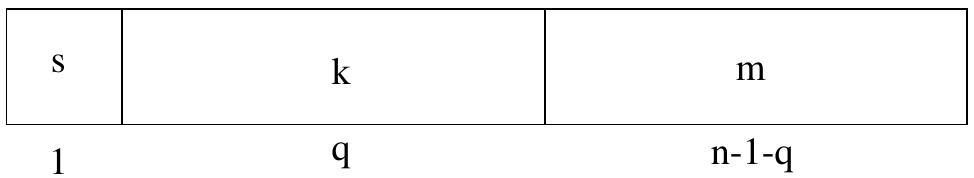
\includegraphics[width=10cm]{figures/ieee_standard.jpeg}
    \end{center}
\end{figure}

\begin{itemize}
    \item Standard IEEE 754.
    \item A number is represented as 
    $$
    f=s.m.b^e
    $$
    $$
    e=k-(2^{q-1}-1); 0\leq m \leq b
    $$
    \item Floats: $m=23$, $e=8$, $s=1$
    \item Doubles: $m=52$, $e=11$, $s=1$
\end{itemize}

\framebreak
{\large Special Cases}
\topline

\begin{itemize}
    \item The standard also defines 3 extra numbers: NaN, $-\inf$ and $+\inf$.
    \item It uses the two extremes of the exponent to represent them.
\end{itemize} 

There are lot of more on the floating point numbers to study.
\emph{http://docs.oracle.com/cd/E19957-01/806-3568/ncg\underline{ }goldberg.html}. We may take one class specially for that topic if you're interested.

\end{frame}


\begin{frame}[allowframebreaks]{C programming Language}
\topline

\begin{minipage}{5cm}

\begin{figure}
    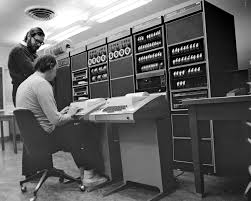
\includegraphics[width=5cm]{figures/richie.jpg}
\end{figure}

\end{minipage}\ \ 
\begin{minipage}{5cm}
{\small
\begin{itemize}
    \item Born in 1972 at Bell labs by Dennis Richie and Ken Thompson.
    \item Initially to develop UNIX.
    \item Normalized by ANSI in 1989: C89 or ANSI C.
    \item Recovered by ISO in 1990: C90.
    \item C99 in 1999 with a lot of new stuff, very close to C++.
    \item New standard C11 in 2011 lots of new stuff.
\end{itemize}
}
\end{minipage}

\framebreak
\topline

{\Large Features}

\begin{itemize}
    \item Compiled language.
    \item Low level language.
    \item Efficient.
    \item Adapted to system operations: direct access to memory and control of low level process.
    \item Require large efforts from developer side.
    \item Reduced standard library.
    \item Not object oriented programming language.
\end{itemize}

\framebreak
\topline

{\Large Compiling}

\begin{figure}
\begin{center}
    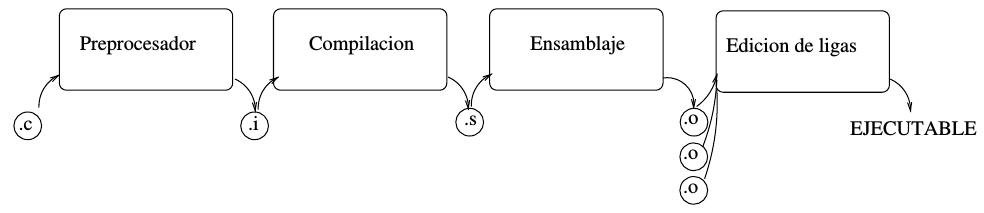
\includegraphics[width=11cm]{figures/building.jpeg}
\end{center}
\end{figure}

\begin{itemize}
    \item Preprocessor: $\#define, \#include$.
    \item Compiling: transforms code into assembly code.
    \item Assembly transforms assembler code into machine code.
    \item Link editing combines object files into one executable.
\end{itemize}


\framebreak
\topline

{\Large Language elements}

\begin{itemize}
    \item Identifiers: variable names, struct names, labels, functions names, etc.
    \item Keywords: type names (*,\&,...), control structures (while, if,...), types classifiers (int, float,...).
    \item Constant names and macros (from preprocessor) included by DEFINE.
    \item Strings.
    \item Operators (+,*,-,...).
    \item Punctuation(;).
    \item Comments.
\end{itemize}

\framebreak
\topline

\begin{itemize}
    \item Expressions: \textbf{int} a; \textbf{double} d;
    \item Variable definition: a=1; d = 2.1*a+a*a;
    \item Integer constants: 
        \begin{itemize}
            \item Decimal: \textbf{int} x =100;
            \item Octal (introduced by 0): \textbf{int} x = 0144;
            \item Hexadecimal (introduced by 0x); \textbf{int} x = 0x64;
        \end{itemize}
   \item Flating constants. By default are double. We can modify them to \textbf{long double} (L) or \textbf{float} (F)
       \begin{itemize}
           \item 12.34 \textbf{double}
           \item 12.3e-4 \textbf{double}
           \item 12.34F \textbf{float}
           \item 12.34L \textbf{long double}
       \end{itemize}
       
\end{itemize}

\end{frame}


\begin{frame}[fragile]{Functions}
\topline

General form

\begin{lstlisting}[language=C++,basicstyle=\ttfamily,keywordstyle=\color{blue}]
type functionname(type1 arg1, type2 arg2,...){
    variable declaration scope;
    instructions;
    return somethingOfTypetype;
}
\end{lstlisting}

\begin{itemize}
    \item Are the structuring base of a program.
    \item At running time they are inside the stack.
    \item main() is the topest function in the stack.
\end{itemize}


\end{frame}


\begin{frame}[fragile,allowframebreaks ]{Operators}
\topline

{\Large Arithmetic}

\begin{itemize}
    \item +,-,*,/,\%.
    \item lvalue: is a value to which we can assign a memory address.
    \item rvalue: are typically operation results.
    \item Relation operators: $>,<,<=,>=,==,!=$
\end{itemize}

\framebreak
\topline

{\Large Logic}

\begin{itemize}
    \item \&\&: AND, $||$ : OR, !: NOT.
    \item The evaluation returns \textbf{int} the value of 1 means true, 0 for false.
    \item Left to right evaluation in case of a group of expressions.

\begin{lstlisting}[language=C++,basicstyle=\ttfamily,keywordstyle=\color{blue}]
if ( (i>=0) && (i<=9) && 
     !(a[i] == 0) || (a[i]>3) ){
     ....
\end{lstlisting}

\framebreak
\topline

    \item Think about the order, better to stand in the following way to gain efficiency

\begin{lstlisting}[language=C++,basicstyle=\ttfamily,keywordstyle=\color{blue}]
if ( mostFrecuentlyViolatedCondition && ... &&
     lessFrecuentlyViolatedCondition ){
     ....
\end{lstlisting}

\end{itemize}

\framebreak
\topline

{\Large Bitwise logic operator}

\begin{itemize}
    \item \&: AND, $|$ : OR, $\sim$: NOT, \^\  :XOR.
    \item $>>,<<$ shift over the bits to the left and to the right. Add zeros at the end or to the right.
    \item These are not boolean operators
\end{itemize}

\framebreak
\topline


{\Large Applications}

\begin{itemize}
    \item Hint: use these operators only to unsigned type data.
    \item Multply or divide by power of two.
\end{itemize}

\end{frame}

\end{document}